\documentclass{article}

\usepackage{amsmath}
\usepackage{amssymb}
\usepackage{amsfonts}
\usepackage{mathtools}

\usepackage[thmmarks, amsmath]{ntheorem}

\usepackage{graphicx}
\usepackage{float}
\usepackage{tikz-cd}
\usepackage{adjustbox}

\usepackage{diffcoeff}
\diffdef{}{op-symbol=\mathrm{d},op-order-sep=0mu}

\usepackage{cancel}
\usepackage{interval}

\usepackage{array}

\usepackage{enumitem}

\setlist[enumerate,1]{label=(\alph*)}

\title{Algebraic Topology Final}
\author{Duarte Maia}
%\date{}

\theoremstyle{plain}
\theorembodyfont{\upshape}
\theoremseparator{.}
\newtheorem{theorem}{Theorem}
\newtheorem{prop}{Prop}
\renewtheorem*{prop*}{Prop}
\newtheorem{lemma}{Lemma}
\newtheorem*{ex}{Exercise}

\theoremstyle{nonumberplain}
\theoremheaderfont{\itshape}
\theorembodyfont{\upshape}
\theoremseparator{:}
\theoremsymbol{\ensuremath{\blacksquare}}
\newtheorem{proof}{Proof}
\newtheorem{sol}{Solution}

\theoremsymbol{\text{\textit{(End proof of lemma)}}}
\newtheorem{lemmaproof}{Proof of lemma}

\newcommand{\R}{\mathbb{R}}
\newcommand{\C}{\mathbb{C}}
\newcommand{\Z}{\mathbb{Z}}
\newcommand{\Q}{\mathbb{Q}}

\newcommand{\RP}{\mathbb{RP}}

\newcommand{\kk}{\Bbbk}

\newcommand{\PP}{\mathbb{P}}
\newcommand{\FF}{\mathcal{F}}

\newcommand{\I}{\mathrm{i}}
\newcommand{\e}{\mathrm{e}}

\newcommand{\id}{\mathrm{id}}
\newcommand{\GL}{\mathrm{GL}}

\newcommand{\conj}[1]{\overline{#1}}
\newcommand{\close}[1]{\overline{#1}}

\DeclareMathOperator{\interior}{int}
\DeclareMathOperator*{\colim}{colim}
\DeclareMathOperator{\codim}{codim}
\DeclareMathOperator{\trace}{tr}
\newcommand{\grad}{\nabla}


\DeclareMathOperator{\Ext}{Ext}
\DeclareMathOperator{\Hom}{Hom}

\DeclarePairedDelimiter{\abs}{\lvert}{\rvert}
\DeclarePairedDelimiter{\norm}{\lvert}{\rvert}
\DeclarePairedDelimiter{\Norm}{\lVert}{\rVert}
\DeclarePairedDelimiter{\braket}{\langle}{\rangle}


\begin{document}
\maketitle

\begin{ex}[1.3:24]
\leavevmode
\begin{enumerate}
\item Show that every path-connected covering space between $X$ and $X/G$ is isomorphic to $X/H$ for some subgroup $H$ of $G$.
\item Two such covering spaces are isomorphic iff the corresponding subgroups are conjugate.
\item $X/H \to X/G$ is normal iff $H$ is a normal subgroup of $G$, in which case the group of deck transformations of this cover is $G/H$.
\end{enumerate}
\end{ex}

\begin{sol}
In this solution we use the following lemma (lemma A). If $H$ is a subgroup of $G$, then the identification $\pi(X/G)/p_*(\pi(X)) \cong G$ (prop 1.40) maps $p_*(\pi(X/H))/p_*(\pi(X))$ to $H$.

Proof of lemma A: We look closely at the identification. An element $g \in G$ is taken to the path in $X/G$ given as follows: draw a path $\gamma$ from the basepoint $x_0 \in X$ to $g x_0$ and map this path down to $X/G$. (This is just Hatcher stuff, see proposition 1.40.)

Now, the subgroup corresponding to elements $h \in H$ consists only of paths from $x_0$ to elements of $H x_0$. In other words, paths that descend to loops in $X/H$, and only those. In other words, if we descend further to $X/G$, we obtain paths in $p_*(\pi(X/H))$, which completes the proof of the lemma.

\leavevmode
\begin{enumerate}
\item By lemma 1.37 in Hatcher, it suffices to show that there exists some subgroup $H \subseteq G$ such that $p_*(\pi(X/H, [x_0])) = p_*(\pi(Y,y_0))$, where $x_0$ is some basepoint in $X$, brackets means taking equivalence class, $y_0$ is the corresponding basepoint in $Y$, and we're using $p$ for all covering maps at hand because notation is difficult.

Now, we know the following. By proposition 1.40,
\begin{equation}
G \cong \pi(X/G, [x_0])/p_*(\pi(X,x_0)).
\end{equation}

Now, $p_*(\pi(Y,y_0))/p_*(\pi(X,x_0))$ is a subgroup of this thing (note that the quotient is well-defined because $X$ covers $Y$), and by passing through the isomorphism we obtain a subgroup $H$ of $G$.

Now, since $G$ is a covering space action, it is obvious from looking at the definition that $H$ is as well, so the covering space $X/H$ is well-defined. Moreover, $G/H$ acts on this space, and it is also easy to see that this is a covering space action (just build $U$ as you would for the action of $G$ on $X$ and pass to the quotient). As such, there is a covering map $X/H \to (X/H)/(G/H)$, and the latter is naturally homeomorphic to $X/G$. This yields a covering map $X/H \to X/G$.

Finally, let us compute $p_*(\pi(X/H,[x_0]))$. This contains $p_*(\pi(X,x_0))$ because $X$ covers $X/H$. Therefore, it suffices to compute
\begin{equation}
\Gamma = p_*(\pi(X/H, [x_0]))/p_*(\pi(X,x_0)),
\end{equation}
but by lemma A above this is corresponds exactly to $H \subseteq G$ under the identification, and so by definition of $H$ the group $\Gamma$ is precisely $p_*(\pi(Y,y_0))/p_*(\pi(X,x_0))$. Following the first paragraph, this completes the solution.

\item Let $H$ and $H'$ be two subgroups of $G$. Then, by lemma 1.37 the spaces $X/H$ and $X/H'$ are isomorphic as basepointed covering spaces if and only if $p_*(\pi(X/H)) = p_*(\pi(X/H'))$, if and only if $p_*(\pi(X/H))/p_*(\pi(X)) = p_*(\pi(X/H'))/p_*(\pi(X))$. Now, both of these are subgroups of
\begin{equation}
p_*(\pi(X/G))/p_*(\pi(X)) \cong G,
\end{equation}
corresponding by lemma A to $H$ and $H'$. Thus, $X/H$ and $X/H'$ are isomorphic as \emph{basepointed} covering spaces iff $H = H'$.

Now, we may adapt the argument used in the second half of theorem 1.38 to make the following adjustment to proposition 1.37: two (non basepointed) covering spaces are isomorphic iff their $p_*(\pi)$ are in the same conjugacy class. As such, repeating the above argument, we obtain that $X/H$ and $X/H'$ are isomorphic as covering spaces iff $H$ and $H'$ are in the same conjugacy class, as desired.

\item By proposition 1.39, the covering $X/H \to X/G$ is normal iff $p_*(\pi(X/H))$ is a normal subgroup of $\pi(X/G)$. Taking the quotient by $p_*(\pi(X))$, $X/H \to X/G$ normal implies that
\begin{equation}
p_*(\pi(X/H))/p_*(\pi(X)) \text{ normal subgroup of } \pi(X/G)/p_*(\pi(X)),
\end{equation}
which by lemma A is equivalent to saying that $H$ is a normal subgroup of $G$.

To prove the other equivalence it suffices to see that the `implies that' above is actually an equivalence. To do this we prove the following algebraic lemma:

Let $f \colon G_1 \to G_2$ be a surjective group homomorphism, and let $H$ be a subgroup of $G_1$ which contains the kernel of $f$. Then, $H$ is normal iff $f(H)$ is normal.

Proof of lemma: ($\rightarrow$) Let $f(g) \in G_2$ and $f(h) \in f(H)$. Then, $f(g) f(h) f(g)^{-1} = f(g h g^{-1}) \in H$ because $H$ is normal. Hence $f(H)$ is closed under conjugation.

($\leftarrow$) Let $g \in G$, $h \in H$. Then we wish to show that $g h g^{-1} \in H$. To do so, note that $f(g h g^{-1}) \in f(H)$, so $f(g h g^{-1}) = f(h')$ for some $h' \in H$. Hence, $g h g^{-1} (h')^{-1} \in \ker f \subseteq H$, and from this it is easy to conclude that $g h g^{-1} \in H$. This completes the proof of the lemma, and hence the solution of the exercise.
\end{enumerate}
\end{sol}

\begin{ex}[3.2:6]
Use cup products to compute the map $H^*(\C P^n; \Z) \to H^*(\C P^n; \Z)$ induced by the map induced from the map $\C^{n+1} \to \C^{n+1}$ obtained by raising every component to the $d$-th power.
\end{ex}

\begin{sol}
We know that $H^*(\C P^n; \Z) \cong \Z[\alpha]/\alpha^{n+1}$, with $\abs{\alpha} = 2$. Thus, it suffices to compute what this map does to $\alpha$, because it generates the cohomology as a ring.

Now, because the homology groups of $\C P^n$ are all free (see page 140) we know that $H^2(\C P^n;\Z)$ is naturally isomorphic to $H_2(\C P^n)^*$, and in turn, since $H_2 \cong \Z$, it suffices to see what the $d$-th power map does to the generator of $H_2(\C P^n)$.

This generator can be obtained by cellular homology, and it is the image under the inclusion of the generator of $\C P^1 \subseteq \C P^n$, hence why Hatcher suggests to do the case $n = 1$ first. Anyway, it then suffices to see what our map does to this generator of $H_2(\C P^1)$.

Okay, well, $\C P^1 = S^2$, as can be easily seen by the $CW$ structure. As such, we can see what our map does to the generator by looking at its degree, which in turn may be computed locally. As such, we compute the degree of the power-$d$ map $\C P^1 \to \C P^1$ locally around the point $[1:0]$. Any nearby point may be represented uniquely as $[1:z]$ with $z \in \C$, and is taken to $[1:z^d]$. This winds around $[1:0]$ $d$ times, and so we conclude that the degree of this map is $d$.

Now we can wind back. This map takes the generator of $H_2(\C P^1)$ to $d$ times itself, so it does the same in $H_2(\C P^n)$, so it does the same in the dual and hence in cohomology. As such, the induced map in cohomology maps $\alpha$ to $d \alpha$, which determines it in the cohomology ring.
\end{sol}

\begin{ex}[3.3:11]
Show that degree 1 maps $f \colon M_g \to M_h$ exist iff $g \geq h$.
\end{ex}

\begin{sol}
If $g \geq h$ this map is easy to construct. First, consider the CW complex of $M_g$ obtained by considering a $4g$-gon. Then, collapse $g-h$ groupings of $4$ edges to obtain a $4h$-gon. This is a map from $M_g$ to $M_h$ which has degree one, because it is the identity on the two-skeleton-modulo-one-skeleton, and so the corresponding map in cellular homology is the identity in second degree.

Now, suppose such a map $f$ exists. Then, note that it preserves the cap product, as in the start of page 241. As such, $[M_g] \cap \alpha = f_*([M_h]) \cap \alpha = f_*([M_h] \cap f^*(\alpha))$ (this uses degree one-ness of $f$). In other words, the following diagram commutes.
\begin{tikzcd}
H^k(M_g;\Z) \arrow[r, "D"]                  & H_{2-k}(M_g) \arrow[d, "f_*"] \\
H^k(M_h;\Z) \arrow[r, "D"] \arrow[u, "f^*"] & H_{2-k}(M_h)                 
\end{tikzcd}

Since the bottom side is an isomorphism, $f_*$ must be surjective in every degree, in particular in $k = 1$. Thus we have a surjective map $\Z^{2g} \to \Z^{2h}$, which by rank arguments shows that $g \geq h$, as desired.
\end{sol}

\begin{ex}[3.3:29]
Show that if $M_g$ retracts onto a graph $X \subseteq M_g$ then $H_1(X)$ has rank at most $g$.

From this show that there is no retraction $M_g \to M'_h$ if $h > g/2$.

Construct a retraction of $M_g$ onto a wedge of $k$ circles with $k \leq g$.
\end{ex}

\begin{sol}
If $M_g$ retracts onto $X$, then the induced map in homology is surjective, as $r \circ i = \id_X$, and hence $r_* \circ i_* = \id$. In particular this is the case in first homology, hence $r_*$ is a surjective map $H_1(M_g) \to H_1(X)$, that is, $\Z^{2g} \to \Z^k$ and thus $k \leq 2g$.

Let $r \colon M_g \to X$ be a retraction, and let $X$ have homology given by $\Z^k$ for some $k$. Then, $r$ induces a map $r^*$ in cohomology, and let us take cohomology over a field $F$, so that cohomology is just the dual of homology. Then we have a ring homomorphism
\begin{equation}
r^* \colon H^*(X) \to H^*(M_g).
\end{equation}
(I will not be writing $F$, but there should be $F$ in every cohomology.)

Okay, now consider the cup product as a map $H^1(M_g) \times H^1(M_g) \to H^2(M_g)$. Recall that the latter is one-dimensional, so we may see the cup product as a bilinear form on $H^1(M_g)$. Moreover, it is skew-symmetric, because $(-1)^{1 \times 1} = -1$. Finally, it is nondegenerate by proposition 3.38 in Hatcher.

Now, let $i$ be the inclusion $X \to M_g$. Then we have $r \circ i = \id_X$, hence $i^* \circ r^* = \id$. As such, $r^*$ is injective, and we may see $H^1(X)$ as a subspace of $H^1(M_g)$, as the image of $r^*$. But now we note that the cup product vanishes on this subspace, because
\begin{equation}
r^*(\alpha) \cup r^*(\beta) = r^*(\alpha \cup \beta) = r^*(0) = 0.
\end{equation}

Thus, we have reduced the problem to showing that a nondegenerate skew-symmetric form $\omega$ on a finite dimensional space $V$ can only vanish on subspaces of dimension up to $\dim V / 2$.

So, let $W \subseteq V$ be a subspace of dimension greater than $\dim V / 2$. Let $V_0$ be a complement of $W$. Note that
\begin{equation}
\dim V_0 = \dim V - \dim W < \dim V - \frac{\dim V}2 = \frac{\dim V}2 = \dim W.
\end{equation}

Moreover, note that $\omega$ induces a linear map $W \to V_0^*$. This map is injective, because for any $w \in W$ there exists some $v \in V$ such that $\omega(w,v) \neq 0$, and since $\omega$ vanishes on $W$ we may write $v = v_0 + w_0$ and we have $\omega(w,v_0) = \omega(w,v) \neq 0$. Anyhow, this is a contradiction because the dimension of $V_0^*$, which equals the dimension of $V_0$, is less than the dimension of $W$. This completes the proof.

\medskip

Now we show that there is no retraction $M_g \to M'_h$ if $h > g/2$. To do so, it suffices to build a retraction of $M'_h$ to a graph whose first homology has rank $2h$. This is trivial. Indeed, $M'_h$ can be built by taking the $4h$-gon, removing a disk from the center, and then identifying the edges pairwise like in the construction of $M_h$. Now, the $4h$-gon with a circle removed retracts in an obvious way to its boundary, and this induces a retraction of $M'_h$ to the one-skeleton of $M_h$, which is a wedge of $2h$ circles.

\medskip

Finally we build a retraction of $M_g$ to a wedge of $k$ circles with $k \leq g$. It suffices to do the case $k = g$, because a wedge of some number of circles retracts to a wedges of less than that number of circles.

So, see $M_g$ as a $4g$-gon with its edges identified pairwise in the standard way. We will construct a retraction of $M_g$ onto $g$ of its one-cells. We will do it for the particular case of $g = 3$, but the construction obviously generalizes for all $g \geq 1$. The case $g = 0$ is very much evident, as any nonempty space retracts to a point.

In the figure below is represented a $12$-gon, whose edges are identified to make $M_3$. In this figure, three bands are represented, and the points not in these bands are colored grey. Then, we make a retraction $M_3 \to X$ as follows. The bands are retracted to the $1$-cell they contain, the same way $S^1 \times I$ retracts to $* \times I$. Then, all gray points are taken to the sole one-cell.

This function is obviously continuous on each region, and thus induces a continuous function on $M_3$ by the gluing lemma. Since the image of each region is contained in (and maps onto) a wedge of three circles, we have a retraction of $M_3$ to $X \cong (S^1)^{\wedge 3}$.

\begin{figure}[H]
\centering
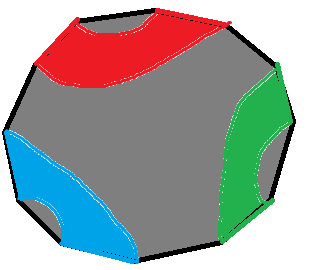
\includegraphics{final1}
\end{figure}
\end{sol}

\begin{ex}[4.2:13]
Show that a map between connected $n$-dimensional CW complexes is a homotopy equivalence if it induces an isomorphism on $\pi_i$ for $i \leq n$.
\end{ex}

\begin{sol}
Let $f \colon X \to Y$ be the map at hand, and let $\tilde X$ and $\tilde Y$ be the universal covers of $X$ and $Y$. Note that $\tilde X$ and $\tilde Y$ are themselves $n$-dimensional CW complexes. Moreover, since $\tilde X$ is simply connected, $f$ lifts to a map $\tilde f \colon \tilde X \to \tilde Y$ such that $p \circ \tilde f = f \circ p$.

Now, note that $p_*$ induces isomorphisms on all $\pi_i$ for $i \geq 2$. As such, by the commutativity property of $\tilde f$, we obtain that $\tilde f$ induces isomorphisms on $\pi_i$ for $2 \leq i \leq n$.

Now, we prove a lemma. Suppose that $f \colon A \to B$ is a map between simply connected spaces which induces isomorphisms in $\pi_i$ for $i \leq n$. Then, it induces isomorphisms in $H_i$ for $i \leq n$.

Proof of lemma: Use the mapping cylinder trick to suppose without loss of generality that $f$ is an inclusion. Then, we may apply the long exact sequence to get exactness of stuff like
\begin{equation}
\pi_k(A) \to \pi_k(B) \to \pi_k(B,A) \to \pi_{k-1}(A) \to \pi_{k-1}(B)
\end{equation}

Now, since the left and right-most maps are isomorphisms, we conclude that $\pi_k(B,A) = 0$ for $k = 1, \dots, n$. As such, we may apply theorem 4.32 to conclude that $H_k(B,A) = 0$ for these values of $k$.

Now, we apply the long exact sequence in homology, which gives us that the following sequence is exact
\begin{equation}
H_k(B,A) \to H_{k-1}(A) \to H_{k-1}(B) \to H_{k-1}(B,A)
\end{equation}
where the middle map, which is therefore an isomorphism for $k \leq n$, is induced by the inclusion $f$. This concludes the proof of the lemma, except for the $n$th homology, which I do not know how to deal with.

Applying this lemma to $\tilde f$, we get that it induces isomorphisms in all homologies up to $n$. Moreover, since $\tilde X$ and $\tilde Y$ are $n$-dimensional cell complexes, their cellular homologies of degree greater than $n$ are all null, and so $\tilde f$ induces an isomorphism on those too. As such, by corollary 4.33, $\tilde f$ is a homotopy equivalence. Thus, it induces isomorphisms on all $\pi_k$. Now, using the fact that the covering maps are isomorphisms on $\pi_k$ for $k \geq 2$ and the commutativity property we talked about in the first paragraph, we conclude that $f \colon X \to Y$ induces isomorphisms on all $\pi_k$, and so by the Whitehead theorem $f$ itself is a homotopy equivalence and the exercise is complete.

\end{sol}

\begin{ex}[4.2:25]
For $X$ a connected CW complex with $\pi_i(X) = 0$ for $1 < i < n$, show that $H_n(X)/h(\pi_n(X)) \cong H_n(K(\pi_1(X),1))$.
\end{ex}

\begin{sol}
Not doing this one.

For the sake of partial credit, here is what little I've gathered. Let $\tilde K$ be the universal cover of $K = K(\pi_1(X),1)$. By hypothesis, $\tilde K$ is contractible, hence $\pi_n(\tilde K) = 0$, and by proposition 4.1 we have that $\pi_n(K) = 0$ for $n > 1$.
\end{sol}

\end{document}